
\documentclass[11pt]{article}
\usepackage{graphicx}
\usepackage{listings}
\usepackage{multirow}
\usepackage[english]{babel}
% Titre complet
\title{Report}

\author{Anna Liednikova}


\begin{document}


\section{Introduction}

 
This project was set within the framework of a collaboration with the ALIAE startup where the aim is to develop a chatbot to collect information from clinical patients. The main idea is to replace strictly defined surveys by a more natural conversation in order to let users express themselves freely so that more information could be collected. First, we should be able to analyse the user utterances (does the user speaks about pain, physical activity etc. ?) and detect at least one most probable intent of user message so that chatbot could choose the right strategy for fulfilling information.


A small manually annotated dataset (roughly 100 sentences for each category) was available. So the purpose of the project is to find word embeddings that will allow to expand it by external data using the existing dataset with labelled intents.

We have tried models for sentence representation by word and the whole context in order to use semi-supervised learning by gradually increasing train data by labelling external sources.

\section{Literature review}

James Ferguson et al faced a similar problem with a small labelled dataset. In their article they describe the approach of automatically expanding dataset and improving the performance of baseline models, that was event trigger identification system in their case.

First, they trained a baseline classifier on available data. Then they identified clusters of additional data to obtain grouped paraphrases inspired by the NewsSpike idea introduced in Zhang et al. (2015). After they labelled clusters with baseline model trained fully-supervised. Combining new labelled data and original one they retrained the event extractor. (Semi-Supervised Event Extraction with Paraphrase Clusters: http://aclweb.org/anthology/N18-2058)



\section{Methodology}

sentence representation, clustering , classification



\subsection{Sentence representation models}

\subsubsection{By Word representation}

The most popular word-basis techniques to represent sentences are LDA (Latent Dirichlet Allocation) and Word2Vector model. We used their implementation from gensim library in order to build models based on the initial labelled dataset.

\subsubsection{By Sentence representation}

In order to use context of words more PositionwiseFeedForward and BiLSTM neural networks were implemenent on Pytorch.



\subsection{Clustering models}

The main idea behind using clustering models for evaluating sentence representations is to detect whatever sentences with the same intent populate the same clusters.

For these purposes following clustering models were used: 
\begin{itemize}
\item K-Means (KM)
\item AgglomerativeClustering(‘ward’) (AG)
\item GaussianMixture (GM)
\end{itemize}

The number of clusters was set to the number of intents (20) that allows using not only purity and Silhouette coefficients to evaluate the clusters but also homogeneity and completeness to get the idea how resulting groups correlate with initial intents. Also, for each model, we plotted a confusion matrix with a background gradient to visualize how well clusters separate different intents.



\subsection{Classification models}

SVC on labelled data

test on unlabelled data

\section{Datasets}

\subsection{Dataset with intents}

The initial dataset is created manually covering 20 main possible users intents. Each sentence represents one intent. For, example,

\begin{lstlisting}
{'text': 'After sleep, for 2-3 hours, 
I am better and then start feeling tired again',
 'intent': 'sleep',
}
\end{lstlisting}

Distribution of labels is show on fig. \ref{figure:name}

 \begin{figure}[h]
 	\centering
 	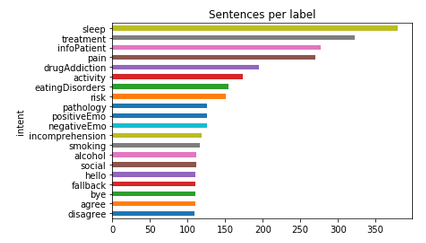
\includegraphics[scale=0.5]{report1.png}
	\caption{Label distribution in dataset}
 \label{figure:name}
 \end{figure}


{'min': 0, 'max': 12, 'mean': 3.438, 'std': 2.16367}

 \begin{figure}[h]
 	\centering
 	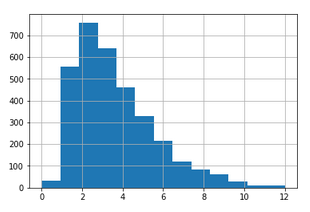
\includegraphics[scale=0.4]{report4.png}
	\caption{Sentence dist}
 \label{words_freq}
 \end{figure}

Total number of sentences is 3305. Found 1882 words after filtering through stopwords list. 

\subsection{Forum data}

To improve initial classifier we needed to extend dataset by much more data and more naturally constracted one. No  test  set  is  available was available at the beginning of the project. To  solve this  problem,  we  opted  to  created  our  own  test set following Zhang et al (2015) and Sondhi et al (2010) example.  

Finally, 272552 unique posts


\subsection{Preprocessing routine}

Some proprocessing routine should be covered. This routine includes sentence tokenization, word tokenization, stop words removing and lemmatization. 

Most popular and common tools for nlp are NLTK and SpaCy but they differ in behaviour.


For example, in word tokenization they give different results that can influence not only simple statistics but meaning too. Some example of different tokenization can be seen in table \ref{token_dif}. Though concating words to ones like 'flulike' or '35mg' or 'longterm' sometimes gives more robust and concrete meaning in case of big dataset, in our case it seems better to stay with spacy way of tokenization in order to have smaller and more simple vocabualary.

For stopwords removing there were three options: nltk, spacy and the longest one. The last option was rejected due to containing words like 'want', 'stop', 'successfully' etc. that can be useful for detecting basic intents like positive or negative emotion, social. Finally nltk one was selecting because of containing shorts like 'm' from 'am', 've' from 'have'. Final dictionary contained 1882 words. Also all numbers were changed to num. Chart (\ref{words_freq}) looks fine.

 \begin{figure}[h]
 	\centering
 	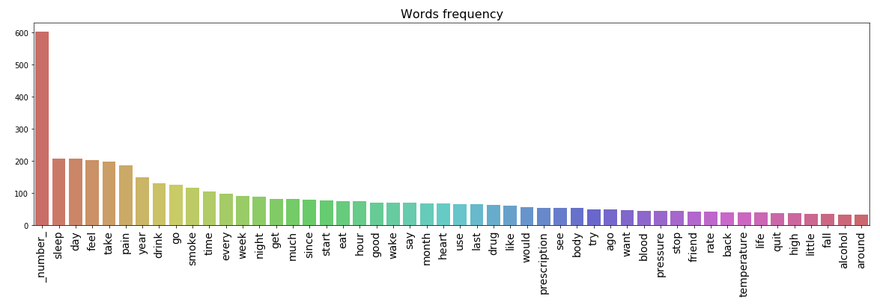
\includegraphics[scale=0.4]{report2.png}
	\caption{Words frequency}
 \label{words_freq}
 \end{figure}

Length < 30.


Next problem is empty sentences. But they don't change the dataset much.

intent
fallback           12
disagree           11
hello               4
agree               3
incomprehension     2
positiveEmo         1

array(['what?', 'same that again', 'I am up', 'same', 'can you',
       'do that', 'do this', 'Will do', 'no', 'no i will not',
       "No i don't", 'no', 'no i will not', "No i don't", "What's up?",
       "What's up?", 'he', 'a', 'd', 'i', 'm', 'o', 's', 't', 'y',
       'I will', 'Will do', 'No', 'no', 'No it is not', "No I don't",
       'No', "I'm here"], dtype=object)

\begin{center}
\begin{table}
\begin{tabular}{ |p{7cm}|p{7cm}| }
\hline
NLTK & SpaCy \\ \hline
['i', 'wouldnt', 'go', 'to', 'sleep', 'until', 'like', '5', '6', 'or', '8am'] & 
['i', 'would', 'nt', 'go', 'to', 'sleep', 'until', 'like', '5', '6', 'or', '8', 'am'] \\ \hline
['that', 'is', 'totally', 'wrongheaded'] & ['that', 'is', 'totally', 'wrong', 'headed'] \\ \hline
['i', 'am', 'in', 'the', 'process', 'of', 'tapering', 'from', 'suboxone', 'longterm', 'use'] & 
['i', 'am', 'in', 'the', 'process', 'of', 'tapering', 'from', 'suboxone', 'long', 'term', 'use'] \\ \hline
['i', 'had', 'an', 'onandoff', 'opiateopioid', 'habit', 'from', 'about', '2010'] & 
['i', 'had', 'an', 'on', 'and', 'off', 'opiate', 'opioid', 'habit', 'from', 'about', '2010'] \\ 
\hline
['i', 'have', 'flulike', 'pathologysymptom'] & ['i', 'have', 'flu', 'like', 'pathologysymptom'] \\ \hline
['i', 'have', 'exerciseinduced', 'insomnia'] & ['i', 'have', 'exercise', 'induced', 'insomnia'] \\ \hline
['i', 'm', 'supposed', 'to', 'take', '6', '35mg', 'tablets', 'a', 'day', 'but', 'i', 'have', 'taken', '20', 'today'] & 
['i', 'm', 'supposed', 'to', 'take', '6', '35', 'mg', 'tablets', 'a', 'day', 'but', 'i', 'have', 'taken', '20', 'today'] \\ 
\hline
\end{tabular}	
\caption{\label{token_dif}Tokenization comparision}
\end{table}
\end{center}



HealthBoards is a medical forum web portal that allows patients to discuss their ailments.
We scraped 272553 unique posts contained in each category. Finally, the corpus consists of N  sentences. Table \ref{visina8} shows the dataset statistics.


{'min': 0, 'max': 2027, 'mean': 10.932588521491454, 'std': 8.964716092053479}
{'min': 3.2580388329566468, 'max': 35.23600634007455, 'mean': 11.224462266261876, 'std': 6.963225985041148}


 \begin{figure}[h]
 	\centering
 	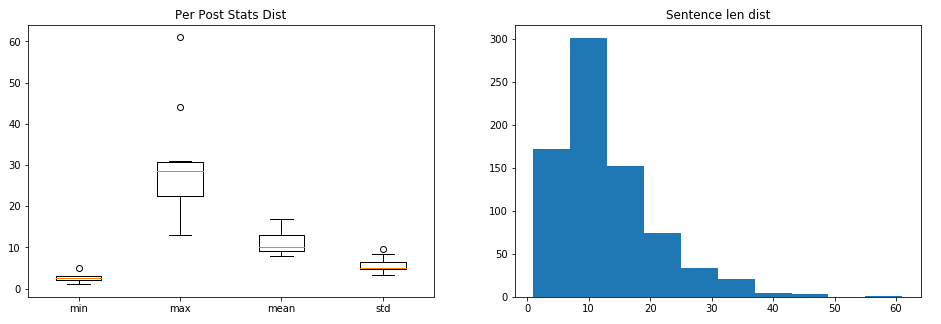
\includegraphics[scale=0.5]{report3.png}
	\caption{Text stat}\label{visina8}
 \end{figure}

Data should be divided in subsets by increasing sentence length because of the difference in mean values for both datasets.



\section{Experiment}

\subsection{Clustering}
\subsubsection{Evoluation metrics}
\subsubsection{W2V model}

Comparision table

\begin{tabular}{ |p{2cm}|p{1cm}|c|c|c|c|p{1cm}| }
\hline
WE & Cluster & purity & Silhouette & homogeneity & complete & Clf CV score \\ \hline
\multirow{3}{*}{Defenders} & KM & & & & &\\
 & AC & & & & &\\
 & GM & & & & &\\ \hline
\multirow{3}{*}{M} & KM & & & & &\\
 & AC & & & & &\\
 & GM & & & & &\\ \hline
Forward & FW & & & & &\\ \hline
\multirow{3}{*}{S} & KM & & & & &\\
 & AC & & & & &\\
 & GM & & & & &\\
\hline
\end{tabular}


\subsubsection{LDA model}


\subsubsection{GloVe pretrained}

\subsubsection{Google News W2V pretrained}

\subsubsection{CNN by word}

From simple encoder, w2v, lda, w2v + lda

\subsubsection{BiLSTM by word}

From simple encoder, w2v, lda, w2v + lda

\subsubsection{Overall comparision}

\subsection{Classifier}
\subsubsection{Evoluation metrics}
\subsubsection{Results for each model}


\section{Conclusion}


\section{References}

@InProceedings{N18-2058,
  author = 	"Ferguson, James
		and Lockard, Colin
		and Weld, Daniel
		and Hajishirzi, Hannaneh",
  title = 	"Semi-Supervised Event Extraction with Paraphrase Clusters",
  booktitle = 	"Proceedings of the 2018 Conference of the North American Chapter of the Association for Computational Linguistics: Human Language Technologies, Volume 2 (Short Papers)",
  year = 	"2018",
  publisher = 	"Association for Computational Linguistics",
  pages = 	"359--364",
  location = 	"New Orleans, Louisiana",
  url = 	"http://aclweb.org/anthology/N18-2058"
}

@InProceedings{sondhi-EtAl:2010:POSTERS,
  author    = {Sondhi, Parikshit  and  Gupta, Manish  and  Zhai, ChengXiang  and  Hockenmaier, Julia},
  title     = {Shallow Information Extraction from Medical Forum Data},
  booktitle = {Coling 2010: Posters},
  month     = {August},
  year      = {2010},
  address   = {Beijing, China},
  publisher = {Coling 2010 Organizing Committee},
  pages     = {1158--1166},
  url       = {http://www.aclweb.org/anthology/C10-2133}
}


@article{article,
author = {Zhang, Thomas and H D Cho, Jason and Zhai, Chengxiang},
year = {2015},
month = {03},
pages = {},
title = {Understanding User Intents in Online Health Forums},
volume = {19},
journal = {IEEE journal of biomedical and health informatics},
doi = {10.1109/JBHI.2015.2416252}

}

\paragraph{APA}

Zhang, T., Cho, J. H. D., \& Zhai, C. (2015). Understanding User Intents in Online Health Forums. IEEE Journal of Biomedical and Health Informatics, 19(4), 1392-1398. [7066225]. https://doi.org/10.1109/JBHI.2015.2416252

\paragraph{Harvard}

Zhang, T, Cho, JHD \& Zhai, C 2015, 'Understanding User Intents in Online Health Forums' IEEE Journal of Biomedical and Health Informatics, vol. 19, no. 4, 7066225, pp. 1392-1398. https://doi.org/10.1109/JBHI.2015.2416252


\end{document}
